%%%%%%%%%%%%%%%%%%%%%%%%%%%%%%%%%%%%%%%%%
% Short Sectioned Assignment LaTeX Template Version 1.0 (5/5/12)
% This template has been downloaded from: http://www.LaTeXTemplates.com
% Original author:  Frits Wenneker (http://www.howtotex.com)
% License: CC BY-NC-SA 3.0 (http://creativecommons.org/licenses/by-nc-sa/3.0/)
%%%%%%%%%%%%%%%%%%%%%%%%%%%%%%%%%%%%%%%%%

%----------------------------------------------------------------------------------------
%	PACKAGES AND OTHER DOCUMENT CONFIGURATIONS
%----------------------------------------------------------------------------------------

\documentclass[paper=a4, fontsize=11pt]{scrartcl} % A4 paper and 11pt font size
% ---- Entrada y salida de texto -----

\usepackage[T1]{fontenc} % Use 8-bit encoding that has 256 glyphs
\usepackage[utf8]{inputenc}
%\usepackage[default]{sourcesanspro}
\usepackage{fourier} % Use the Adobe Utopia font for the document - comment this line to return to the LaTeX default
% ---- Idioma --------

\usepackage[spanish, es-tabla]{babel} % Selecciona el español para palabras introducidas automáticamente, p.ej. "septiembre" en la fecha y especifica que se use la palabra Tabla en vez de Cuadro

% ---- Code insertion ----
\usepackage{minted}
\usepackage[breakable]{tcolorbox} %Genera boxes, lo usamos para el codigo
\BeforeBeginEnvironment{minted}{\begin{tcolorbox}[breakable]}%
	\AfterEndEnvironment{minted}{\end{tcolorbox}}%
\BeforeBeginEnvironment{inputminted}{\begin{tcolorbox}[breakable]}%
	\AfterEndEnvironment{inputminted}{\end{tcolorbox}}%

\usepackage{xpatch} %permite abrir environments al ejecutar ciertos comandos

\xpretocmd{\inputminted}{\begin{tcolorbox}}{}{}%
	\xapptocmd{\inputminted}{\end{tcolorbox}}{}{}%

\setminted{
fontsize=\small,
breaklines,
breaksymbolleft=
}
% ---- Otros paquetes ----
\usepackage{dirtree}
\usepackage{vmargin}

\usepackage{url} % ,href} %para incluir URLs e hipervínculos dentro del texto (aunque hay que instalar href)
\usepackage{hyperref} % ,href} %para incluir URLs e hipervínculos dentro del texto (aunque hay que instalar href)
\hypersetup{
	colorlinks=true,
	linkcolor=blue,
	filecolor=magenta,      
	urlcolor=blue,
}

\usepackage{xcolor}
\definecolor{light-gray}{gray}{0.95}
\definecolor{alizarin}{rgb}{0.82, 0.1, 0.26}
\definecolor{nyellow}{rgb}{0.91, 0.656, 0.0}
%\definecolor{indigo}{rgb}{0.29, 0.0, 0.51}
%	\textcolor{red}{p}
%	\textcolor{orange}{r}
%	\textcolor{yellow}{a}
%	\textcolor{green}{c}
%	\textcolor{blue}{t}
%	\textcolor{indigo}{i}
%	\textcolor{violet}{c}
%	\textcolor{red}{a}
%	\textcolor{orange}{s}
%	\textcolor{yellow}{,}
%	\textcolor{green}{I}
%	\textcolor{blue}{S}
%	\textcolor{indigo}{E}

\usepackage{amsmath,amsfonts,amsthm} % Math packages
%\usepackage{graphics,graphicx, floatrow} %para incluir imágenes y notas en las imágenes
\usepackage{graphics,graphicx, float} %para incluir imágenes y colocarlas
\usepackage[export]{adjustbox}
\graphicspath{{imagenes/}}

% Para hacer tablas comlejas
%\usepackage{multirow}
%\usepackage{threeparttable}

%\usepackage{sectsty} % Allows customizing section commands
%\allsectionsfont{\centering \normalfont\scshape} % Make all sections centered, the default font and small caps

%Remove warnings
\usepackage{silence}
\WarningFilter{scrartcl}{Usage of package `fancyhdr'}

\usepackage{fancyhdr} % Custom headers and footers
\pagestyle{fancyplain} % Makes all pages in the document conform to the custom headers and footers
\fancyhead{} % No page header - if you want one, create it in the same way as the footers below
\fancyfoot[L]{} % Empty left footer
\fancyfoot[C]{} % Empty center footer
\fancyfoot[R]{\thepage} % Page numbering for right footer
\renewcommand{\headrulewidth}{0pt} % Remove header underlines
\renewcommand{\footrulewidth}{0pt} % Remove footer underlines
\setlength{\headheight}{13.6pt} % Customize the height of the header

\numberwithin{equation}{section} % Number equations within sections (i.e. 1.1, 1.2, 2.1, 2.2 instead of 1, 2, 3, 4)
\numberwithin{figure}{section} % Number figures within sections (i.e. 1.1, 1.2, 2.1, 2.2 instead of 1, 2, 3, 4)
\numberwithin{table}{section} % Number tables within sections (i.e. 1.1, 1.2, 2.1, 2.2 instead of 1, 2, 3, 4)

\setlength\parindent{0pt} % Removes all indentation from paragraphs - comment this line for an assignment with lots of text

\newcommand{\horrule}[1]{\rule{\linewidth}{#1}} % Create horizontal rule command with 1 argument of height

\setmarginsrb{2 cm}{1 cm}{2 cm}{2 cm}{1 cm}{1.5 cm}{1 cm}{1.5 cm} %Aumenta los márgenes

%----------------------------------------------------------------------------------------
%	TÍTULO Y DATOS DEL ALUMNO
%----------------------------------------------------------------------------------------

\title{
	\Huge{Práctica Final} \\\vspace{1cm}
	{Nuevos modelos bioinspirados para el Aprendizaje de Pesos en Características \vspace{1cm} \\
	Sheep Flocks Heredity Model (SFHM)}\hspace{1cm} 
 }   

\author{Yeray López Ramírez	}                             

\renewcommand*\contentsname{hola}

\makeatletter
\let\thetitle\@title
\let\theauthor\@author
\let\thedate\@date
\makeatother

%----------------------------------------------------------------------------------------
% DOCUMENTO
%----------------------------------------------------------------------------------------

\begin{document}
\begin{titlepage}
	\centering
	%\textsc{\LARGE Universidad de Granada}\\[2.0 cm]    
	
\includegraphics[scale = 0.6]{ugr.png}\\[1.0 cm]
	\rule{\linewidth}{0.2 mm} \\[0.4 cm]
	{ \huge \bfseries \thetitle}\\
	\rule{\linewidth}{0.2 mm} \\[1.5 cm]
	
	\begin{minipage}{0.5\textwidth}
		\begin{flushleft} \large
			\theauthor 
			123456789-Z \\
			\href{mailto:fulanito@correo.ugr.es}{fulanito@correo.ugr.es}
		\end{flushleft}
	\end{minipage}~
	\begin{minipage}{0.5\textwidth}
		\begin{flushright} \large
			Curso: 2022-23 \\
			Grupo A, 15:30 - 17:30 (Martes)                   
		\end{flushright}
	\end{minipage}\\[1 cm]
	
	{\small \thedate}\\[1 cm]
	
	\vfill
	
\end{titlepage}


\newpage %inserta un salto de página
\newcommand{\code}[1]{\colorbox{light-gray}{\textcolor{alizarin}{\texttt{#1}}}}
\newcommand{\high}[1]{\colorbox{light-gray}{\textcolor{nyellow}{\texttt{#1}}}}

\tableofcontents % para generar el índice de contenidos

\listoffigures

\listoftables

\newpage

%----------------------------------------------------------------------------------------
%	Cuestión 1
%----------------------------------------------------------------------------------------

\section{Resumen}
La metaheurística propuesta, conocida como ``A new evolutionary algorithm based on sheep flocks heredity models'' (Un nuevo algoritmo evolutivo basado en el modelo de herencia de rebaños de ovejas.), introduce el concepto de Operación Genética Multi-etapa (Multi-Stage Genetic Operation) para mejorar la exploración y explotación de soluciones en el proceso de optimización.

\subsection{Inspiración Metaheurística}
Imaginemos que estamos en un campo con 3 rebaños de ovejas diferentes, cada uno con su pastor. Cada oveja tiene unas características propias que son comunes en su rebaño. En un momento dado, los pastores se despistan y las ovejas acaban mezclandose en un gran rebaño:

\begin{minipage}[t]{0.5\textwidth}
	\centering
	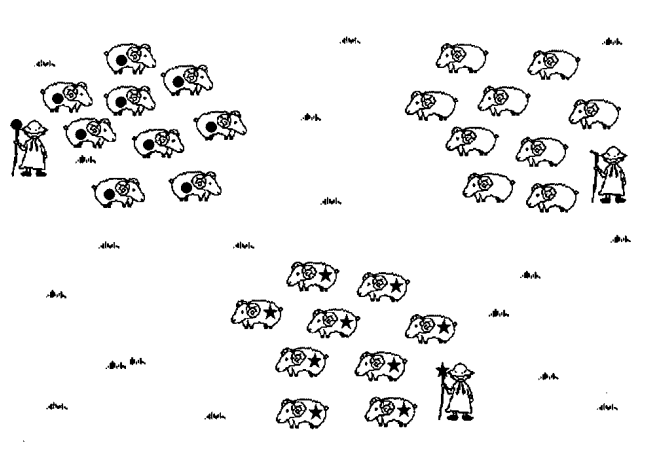
\includegraphics[width=\linewidth]{rebaño1.png}
	\label{fig:rebaño-inicial}
	\captionof{figure}{Las ovejas pastan con su rebaño}
\end{minipage}
\hfill
\vline
\begin{minipage}[t]{0.5\textwidth}
	\centering
	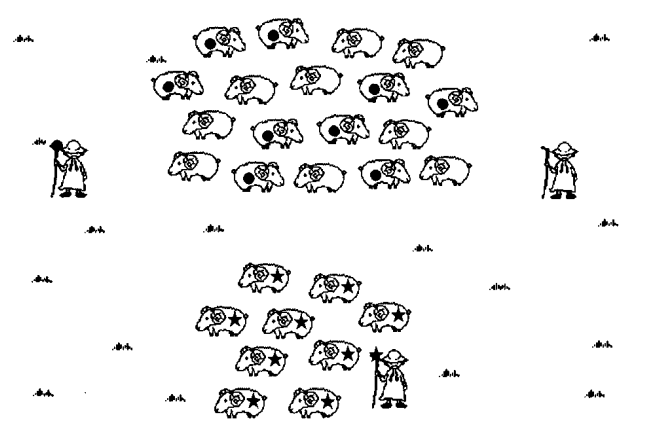
\includegraphics[width=\linewidth]{rebaño2.png}
	\label{fig:rebaño-mezclado}
	
	\captionof{figure}{Las ovejas se mezclan}
\end{minipage}
\quad\\
Cuando se dan cuenta, intentan recoger a sus ovejas pero como no son capaces de diferenciarlas acaban con los 3 rebaños de antes mezclados.
\begin{figure}[H]
	\centering
	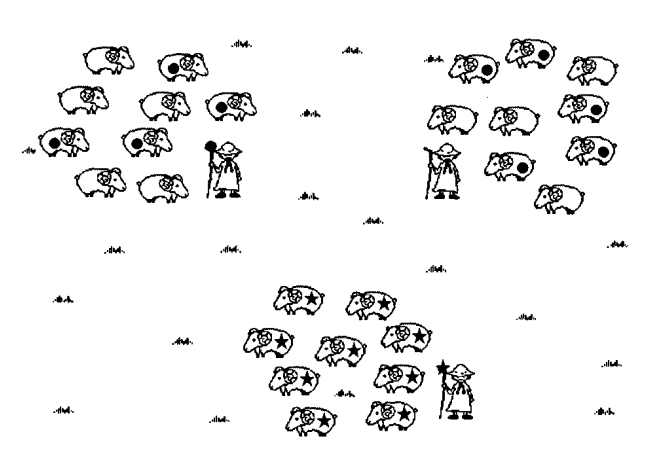
\includegraphics[width=0.5\linewidth]{rebaño3.png}
	\label{fig:rebaño-cruzado}
	\caption{Los pastores recogen a las ovejas y los rebaños quedan mezclados}
\end{figure}
Finalmente cada rebaño se reproduce o desaparece en función del fitness total del rebaño.

\subsection{Correspondencia con el algoritmo real}
Partiendo del ejemplo anterior, vamos a relacionar cada elemento con su forma real. Viene ilustrado en la siguiente tabla:

\begin{table}[h]
	\centering
	\begin{tabular}{|c|c|}
		\hline
		\textbf{Evolución Natural}          & \textbf{Operación Genética Multi-etapa} \\ \hline
		Rebaño                     & Cadena (Cromosoma)             \\ \hline
		Oveja                      & Subcadena (Gen)                \\ \hline
		Mezclado y separado        & Cruce de cromosomas            \\ \hline
		Herencia dentro del rebaño & Cruce de genes                 \\ \hline
	\end{tabular}
\end{table}

En esta metaheurística, cada posible solución se representa como una cadena, donde cada gen de la cadena corresponde a una parte específica de la solución. Esto se asemeja al comportamiento natural de un rebaño de ovejas, donde el rebaño se considera la cadena completa y cada oveja representa un gen o una subcadena. La evolución natural del rebaño se traduce en la operación genética multi-etapa en el algoritmo propuesto.\\

La operación genética multi-etapa consta de dos fases. En la primera fase, se realiza un cruce de cromosomas, donde se seleccionan aleatoriamente dos cromosomas y se intercambian secciones específicas a partir de una posición determinada. Esta fase combina las características de los cromosomas para explorar diferentes soluciones potenciales.\\

En la segunda fase, se realiza un cruce de genes, donde se seleccionan aleatoriamente dos genes de los cromosomas intercambiados en la fase anterior y se intercambian entre sí a partir de una posición aleatoria. Este proceso de cruce de genes permite explorar y explotar soluciones a un nivel más detallado.\\

Para lograr un equilibrio entre la exploración y la explotación, se utiliza un cruce denominado SPX (Single Point Crossover). El cruce SPX toma una posición aleatoria en dos genes o cromosomas y los intercambia a partir de esa posición. Esta técnica ayuda a diversificar las soluciones exploradas y a aprovechar las soluciones prometedoras encontradas.

\begin{figure}[H]
	\centering
	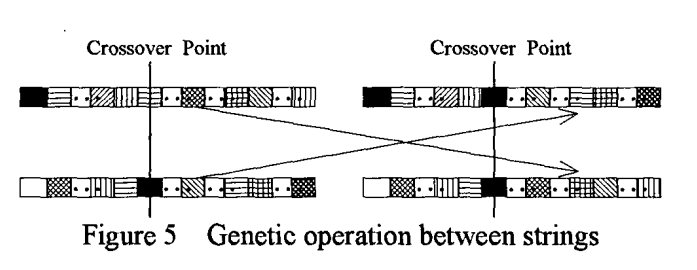
\includegraphics[width=0.6\linewidth]{cruceImagen.png}
	\label{fig:cruce-cromosoma}
\end{figure}

\begin{figure}[H]
	\centering
	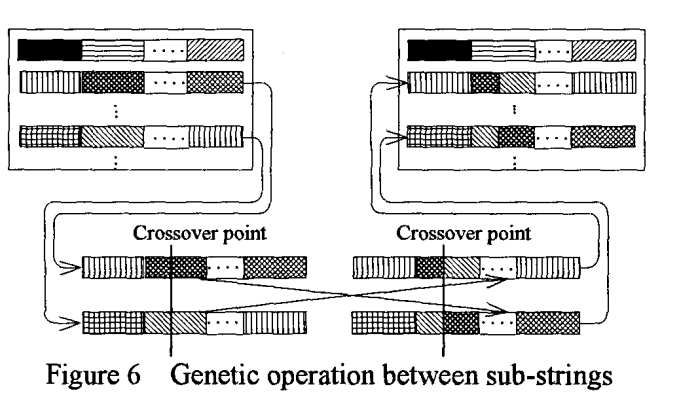
\includegraphics[width=0.6\linewidth]{cruceImagen2.png}
	\label{fig:cruce-gen}
\end{figure}


Esto da como resultado un buen equilibrio entre exploración y explotación. Además, para aumentar aún más la exploración, se introduce la heurística R-R (Robust Replace). La heurística R-R asigna un coeficiente de robustez a cada cromosoma. Si el coeficiente cae por debajo de un umbral predefinido, el cromosoma completo se reemplaza por uno nuevo generado aleatoriamente. Esta estrategia permite descartar soluciones de baja calidad y continuar probando nuevas soluciones en busca de mejores resultados.

\subsection{Fortalezas y debilidades}
El nuevo algoritmo presenta diversas fortalezas y debilidades. Una de sus principales fortalezas es su capacidad para lograr un equilibrio adecuado entre la exploración y la explotación, dando prioridad a la exploración. Esto se logra mediante la incorporación de nuevos operadores y una heurística de exploración al algoritmo genético básico. Además, su implementación resulta sencilla debido a su base en un algoritmo genético simple.\\

Sin embargo, es importante tener en cuenta que existen áreas de mejora en cuanto a su capacidad de explotación. Sería beneficioso incorporar técnicas de Búsqueda Local o Enfriamiento Simulado para mejorar aún más los resultados obtenidos. Otro aspecto que se puede considerar como una debilidad es que el algoritmo tiende a ser más lento en comparación con los algoritmos genéticos convencionales. Esto se debe a la inclusión de la operación de cruce de genes y la heurística de reemplazo R-R.\\

En conclusión, este algoritmo ofrece una alta diversidad de soluciones, lo cual es beneficioso en términos de exploración. No obstante, esto se logra a expensas de una convergencia más lenta y un mayor costo computacional. Para mejorar su rendimiento, sería recomendable considerar la incorporación de técnicas de explotación adicionales y optimizar los aspectos computacionales.

\section{Adaptación al problema de Prácticas APC}
La adaptación del algoritmo Sheep Flock Heredity Model (SFHM) al problema de Prácticas de Aprendizaje de Pesos en Características (APC) tiene como objetivo utilizar las capacidades de optimización del algoritmo genético para encontrar una combinación óptima de pesos de características.\\

En el contexto de las Prácticas APC, el objetivo principal es encontrar una configuración de pesos que maximice la capacidad discriminativa de un clasificador, al tiempo que minimiza la redundancia y el ruido introducido por características irrelevantes.\\

Para adaptar el algoritmo SFHM al problema de APC, se deben realizar las siguientes modificaciones:

\begin{itemize}
	\item Representación de la solución: En el algoritmo SFHM, cada oveja representa una solución en el espacio de búsqueda. En el contexto de las Prácticas APC, la solución debe ser una combinación de pesos para cada característica. Por lo tanto, se debe definir una representación adecuada que permita codificar los pesos de manera eficiente. Por ejemplo, se puede utilizar un vector de valores reales donde cada elemento representa el peso correspondiente a una característica.
	\item Función de evaluación: En las Prácticas APC, la función de evaluación debe medir la calidad de una configuración de pesos en términos de precisión, exactitud o alguna otra métrica de rendimiento del clasificador. Por lo tanto, se debe definir una función de evaluación adecuada que utilice un clasificador entrenado con la configuración de pesos actual para calcular la métrica de rendimiento deseada.
	\item Operadores genéticos: El algoritmo SFHM utiliza operadores genéticos como la reproducción, el cruce y la mutación para evolucionar y mejorar las soluciones. Estos operadores deben ser adaptados para trabajar con la representación de pesos de características. Por ejemplo, el cruce puede combinar los pesos de características de dos padres mediante una técnica como el cruce de un punto o el cruce uniforme. La mutación puede modificar los pesos de características mediante operaciones como el cambio aleatorio de peso o la mutación local basada en vecindarios de características.
	\item Parámetros del algoritmo: Los parámetros del algoritmo, como la probabilidad de mutación y cruce, el tamaño de la población y el número máximo de iteraciones, deben ser ajustados de acuerdo con las características del problema de APC. Estos parámetros afectarán la exploración y explotación del espacio de búsqueda y pueden influir en la calidad de las soluciones encontradas.
	\item Integración de Búsqueda Local: Como se mencionó anteriormente, se puede considerar la hibridación del SFHM con la Búsqueda Local para mejorar la capacidad de explotación del algoritmo. La Búsqueda Local se aplicaría en intervalos regulares para refinar las soluciones encontradas y mejorar aún más su rendimiento.
\end{itemize}

\subsection{Operadores APC}

\textbf{Operador de selección}: se seleccionan de forma aleatoria y sin repetición los individuos de la población

\textbf{Operador de Cruce}: es un algoritmo por el cual 2 individuos ''padres'' de la poblacion son mezclados entre sí para generar 2 ''hijos''. Para nuestro problema se ha utilizado el operador de cruce SPX. El proceso de cruce SPX se lleva a cabo de la siguiente manera:

\begin{itemize}
	\item Selección de padres: Se seleccionan dos cromosomas (o subcromosomas) de la población actual como padres para el cruce.
	\item Selección del punto de cruce: Se elige aleatoriamente un punto de corte en el cromosoma. Este punto de corte divide los cromosomas en dos partes, una antes del punto de corte y otra después del punto de corte.
	\item Intercambio de información genética: A partir del punto de corte seleccionado, se intercambian las porciones correspondientes entre los dos padres para generar la descendencia. Es decir, los genes que se encuentran antes del punto de corte en un padre se copian en la descendencia desde el primer padre, mientras que los genes que se encuentran después del punto de corte se copian desde el segundo padre.
	\item Creación de descendientes: La descendencia generada mediante el intercambio de información genética se convierte en nuevos individuos que formarán parte de la siguiente generación. Puede haber uno o más descendientes generados en cada operación de cruce, dependiendo de la implementación específica del algoritmo genético.
\end{itemize}

Este proceso se repite para un número determinado de veces, produciendo así una nueva generación de individuos que combina características de los padres originales. El objetivo del cruce es explorar y explotar el espacio de búsqueda de soluciones, permitiendo la creación de nuevas soluciones potencialmente mejores a través de la combinación de características prometedoras de los padres.


\begin{algorithm}[H]
	\caption{Cruce de un punto}
	\SetKwInOut{Input}{Entrada}
	\SetKwInOut{Output}{Salida}
	
	\Input{padre1, padre2, punto de cruce}
	\Output{hijo1, hijo2}
	
	\BlankLine
	\BlankLine
	punto cruce = generarNumeroAleatorio(0 hasta el número total de características)\;
	\For{i = 1 hasta el número total de características}{
		\If{i $\leq$ punto de cruce}{
			hijo1[i] $\leftarrow$ padre1[i]\;
			hijo2[i] $\leftarrow$ padre2[i]\;
		}
		\Else{
			hijo1[i] $\leftarrow$ padre2[i]\;
			hijo2[i] $\leftarrow$ padre1[i];
		}
	}
	\BlankLine
	\Return hijo1, hijo2\;
	
\end{algorithm}
\quad\\

\textbf{Operador de Mutación}: se encarga de introducir cambios aleatorios en los individuos seleccionados. Es importante para mantener la diversidad genética en la población y evitar que el algoritmo se estanque en óptimos locales. Veremos 2 tipos de mutación:

\begin{itemize}
	\item \textbf{Mutación Inversa:} Dado un individuo, se invierten uno o más genes de manera aleatoria. La inversión de genes implica cambiar el orden de los genes en una parte del cromosoma. Por ejemplo, si el cromosoma es una cadena de bits ``01101001'' y se invierte la sección que va desde el índice 3 al índice 6, el resultado sería ``01010101''. Su codificación general es:\\
\begin{algorithm}[H]
	\caption{Mutación Inversa}
	\SetAlgoLined
	\SetKwInOut{Input}{Entrada}
	\SetKwInOut{Output}{Salida}
	
	\Input{individuo, tasa de mutación}
	\Output{individuo mutado}
	
	\BlankLine
	\BlankLine

	punto de inicio $\leftarrow$ generar número aleatorio entre [0, longitud del cromosoma]\;
	punto de fin $\leftarrow$ generar número aleatorio entre [punto de inicio, longitud del cromosoma]\;
	\For{i $\leftarrow$ puntoInicio hasta puntoFin}{
		swap $\leftarrow$ individuo[i]\;
		individuo[i] $\leftarrow$ individuo[puntoFin]\;
		individuo[puntoFin] $\leftarrow$ swap\;
		puntoFin $\leftarrow$ puntoFin -1\;
	}
	
	\Return individuo mutado;
	
\end{algorithm}

	\item \textbf{Mutación en un punto:} En el punto de mutación seleccionado, se añade un valor aleatorio al valor del gen. Por ejemplo, si el gen es 0.45, la mutación podría consistir en agregar un valor aleatorio como puede ser 0.3 quedando 0.75 como valor del gen. Su codificación general es:\\
	\begin{algorithm}[H]
		\caption{Mutación en un punto}
		\SetKwInOut{Input}{Entrada}
		\SetKwInOut{Output}{Salida}
		
		\Input{individuo, posAMutar}
		\Output{individuo mutado}
		
		\BlankLine
		valorAMutar = generar distribucion aleatoria (media=0, varianza=sqrt(0.8));\\
		individuo[posAMutar] += z\;
		\If{individuo[posAMutar] $\le$ \ 0.1}{
			individuo[posAMutar] $\leftarrow$ 0.1
		}		
		\If{individuo[posAMutar] $\ge$ \ 1.0}{
			individuo[posAMutar] $\leftarrow$ 1.0
		}
		\BlankLine
		\Return individuo mutado\;
	\end{algorithm}
\end{itemize}




El operador de mutación tiene una tasa de 0.1 de mutar lo que significa que es que se ejecutará solo con el 10\% de la población aleatoriamente. En pseudocódigo se haría:\\
\begin{algorithm}[H]
	\caption{Aplicar mutación}
	\SetKwInOut{Input}{Entrada}
	\SetKwInOut{Output}{Salida}
	
	\Input{poblacion, tasa de mutación}
	\Output{poblacion mutada}
	
	\BlankLine
	\BlankLine
	\For{i = 1 to tamanio de poblacion * tasa de mutacion}{
			individuoAMutar = generar numero aleatorio de rango [0, tamanio de la poblacion]; \\
			posAMutar = generar numero aleatorio de rango [0, numero de caracteristicas];
			\BlankLine
			Mutacion(individuo[individuoAMutar], posAMutar); 
	}
	\BlankLine
	\Return Poblacion mutada\;
\end{algorithm}
\quad\\

\textbf{Operador de Reemplazamiento}: el principal mecanismo de reemplazamiento del algoritmo es la heurística R-R (Robust Replace). Consiste en asignar un valor de coeficiente a cada cromosoma que indique su calidad como puede ser la función de fitness. Si el fitness de ese cromosoma es inferior al fitness medio de la población, es reemplazado por un nuevo cromosoma aleatorio. \\

La implementación final en pseudocódigo es:

\begin{algorithm}[H]
	\caption{Sheep Flock Heredity Model Algorithm}
	\SetKwInOut{Input}{Entrada}
	\SetKwInOut{Output}{Salida}
	
\Input{train, maxIters, operador}
\Output{mejorSolucion}

\BlankLine
\BlankLine

\tcp{Crear población inicial}
Poblacion pop\;
pop $\leftarrow$ nuevas\_soluciones(rebanios, numCaracteristicas)\;

\While{iter $<$ maxIters}{
	\tcp{Stage 1 - Operaciones subcromosoma}
	
	\tcp{Obtener nuevo padre sin repetición}
	parent $\leftarrow$ getParent(pop)\;
	
	\tcp{Cruce subcromosoma}
	\If{Random::get(0.0, 1.0) $\leq$ CROSS\_PER\_CENT}{
		hijo $\leftarrow$ cruceSPX(parent, num\_ovejas, tam\_ovejas)\;
	}
	
	\tcp{Mutación subcromosoma}
	\If{Random::get(0.0, 1.0) $\leq$ MUT\_PER\_CENT}{
		inverseMov(parent)\;
		Mov(parent, VARIANZA)\;
	}
	
	\tcp{Stage 2 - Operaciones Cromosomas}
	
	\tcp{Seleccionar dos padres sin repetición}
	parent1 $\leftarrow$ getParent(pop)\;
	parent2 $\leftarrow$ getParent(pop)\;
	
	\tcp{Cruce cromosoma}
	\If{Random::get(0.0, 1.0) $\leq$ pcross}{
		hijo1, hijo2 $\leftarrow$ cruceSPX(parent2, parent3)\;
	}
	
	\tcp{Mutación cromosoma}
	\If{Random::get(0.0, 1.0) $\leq$ pmut}{
		posi $\leftarrow$ Random::get(1, pop.numCaracteristicas());
		inverseMov(parent2);
		inverseMov(parent3);
		Mov(parent2, VARIANZA);
		Mov(parent3, VARIANZA);
	}

	\tcp{Actualizar los individuos en la población}
	setIndividuo(hijo, pop)\;
	setIndividuo(hijo1, pop)\;
	setIndividuo(hijo2, pop)\;

	\BlankLine
% Incrementar el contador de iteraciones
iter $\leftarrow$ iter + 3\;
}

% Devolver la mejor solución encontrada
\Return mejorIndividuo(pop)\;

\end{algorithm}


\subsection{Hibridación SFHM + BL}
La hibridación del algoritmo SFHM con Búsqueda Local tiene como objetivo mejorar la capacidad de explotación del algoritmo base. La principal deficiencia de SFHM es su enfoque basado en la exploración global del espacio de búsqueda, lo que puede llevar a un menor rendimiento en la explotación de las soluciones encontradas. La integración de Búsqueda Local busca compensar esta deficiencia al aplicar una estrategia de refinamiento local en etapas específicas del algoritmo.\\

En este enfoque híbrido, se decide aplicar la Búsqueda Local cada 10 iteraciones del algoritmo SFHM. Además, se selecciona el 10\% de los individuos con el mejor fitness de la población actual para someterlos a la Búsqueda Local. Esta estrategia es similar a la utilizada en el enfoque Memético-Best, donde se combina la exploración global con la explotación local.\\

La Búsqueda Local consiste en realizar modificaciones locales en las soluciones seleccionadas, con el objetivo de mejorar su calidad. Estas modificaciones se basan en operadores específicos diseñados para el problema en cuestión. En cada iteración de la Búsqueda Local, se exploran y evalúan soluciones vecinas para determinar si mejoran el fitness de la solución actual. Si se encuentra una solución mejor, se actualiza la solución actual con la mejor solución vecina encontrada.\\

La aplicación de la Búsqueda Local en el SFHM + Búsqueda Local permite refinar las soluciones obtenidas durante el proceso de evolución del algoritmo. Esto ayuda a mejorar la calidad de las soluciones finales, ya que se enfoca en la explotación de las regiones prometedoras del espacio de búsqueda.\\

La implementación de la mejora sería:

\begin{algorithm}[H]
	\caption{Hibridación SFHM + BL}
	\SetKwInOut{Input}{Entrada}
	\SetKwInOut{Output}{Salida}
	
	\Input{poblacion}
	\Output{Mejor Solución}
	
	\BlankLine
	
	\tcp{Ejecuta SFHM}
	SFHM(poblacion)\;
	
	mejoresSoluciones = getMejores(0.10) \;
	\For{i hasta 10\% de poblacion}{
		mejoresSoluciones $\leftarrow$ BL(mejoresSoluciones[i])
	}
	
	poblacion $\leftarrow$ actualizarPoblacion(mejoresSoluciones, poblacion)\;
	
	\BlankLine
	\Return Mejor Solucion\;
\end{algorithm}


\subsection{Mejoras}

Para mejorar el algoritmo SFHM, se han investigado papers más recientes que proponen diversas mejoras y adaptaciones al algoritmo original. A continuación, se presentan algunas de estas mejoras:

\begin{enumerate}
	\item Metaheurística R-R (Robust Replace): Se ha propuesto la incorporación de la heurística R-R al algoritmo SFHM \cite{rr}. Esta heurística se utiliza para reemplazar aquellos cromosomas cuyo fitness es inferior a la media de la población. Al aplicar esta estrategia de reemplazo, se busca mejorar la calidad de las soluciones seleccionadas para la reproducción y, potencialmente, acelerar la convergencia del algoritmo.
	\item Mutación adicional: En el paper original de SFHM \cite{ori}, no se incluye la mutación inversa y la mutación en un punto. Sin embargo, en investigaciones más recientes \cite{rr}, se ha propuesto la incorporación de estas mutaciones como parte del proceso evolutivo. La mutación inversa implica invertir el orden de los genes en un cromosoma, mientras que la mutación en un punto consiste en cambiar aleatoriamente el valor de un gen en un cromosoma. Estas mutaciones adicionales aumentan la diversidad genética y la exploración del espacio de búsqueda, lo que puede mejorar la capacidad de encontrar soluciones óptimas.
	\item Mutación pair-wise: En otro paper donde se adapta el algoritmo SFHM al problema de formación de células \cite{pr}, se introduce una mutación denominada "pair-wise mutation". Esta mutación implica realizar modificaciones en pares de genes adyacentes en un cromosoma. La mutación pair-wise se ha diseñado específicamente para el problema de formación de células, pero puede ser explorada y adaptada para otros problemas similares.
\end{enumerate}

Al implementar estas mejoras en el algoritmo SFHM, se espera obtener una mayor capacidad de exploración y explotación del espacio de búsqueda, lo que puede conducir a soluciones de mayor calidad. Además, estas mejoras han sido propuestas y evaluadas en papers científicos, lo que respalda su eficacia en diferentes contextos y problemas específicos.

\section{Resultados Algoritmos Prácticas 1,2,3 y Alternativa}

\begin{figure}[h]
	\centering
	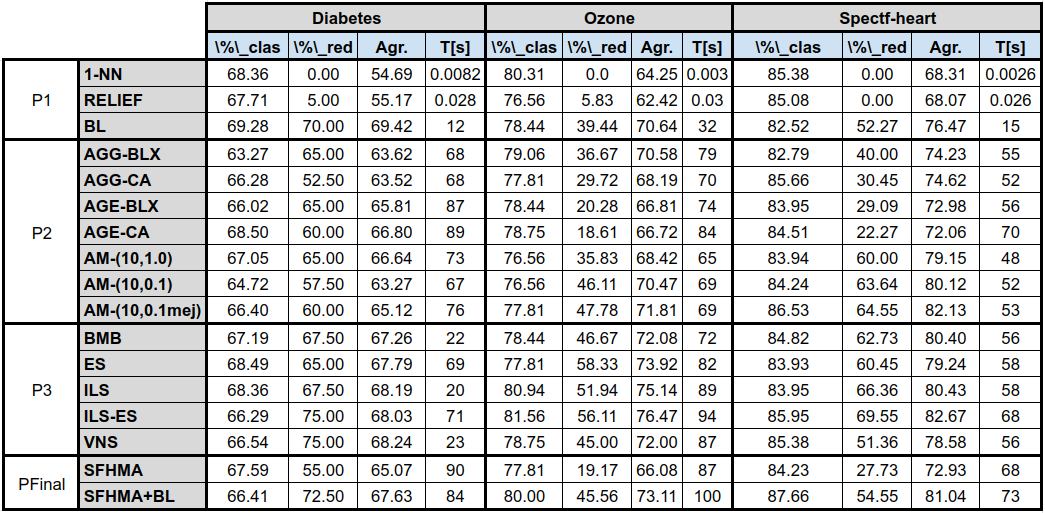
\includegraphics[width=\textwidth]{tablaFinal.png}
	\caption{Resultados obtenidos de todas las prácticas y SFHMA}
	\label{fig:final}
\end{figure}

Para analizar los resultados, se compararon los algoritmos en términos de las tasas de clasificación (\%\_clas), las tasas de reducción (\%\_red), la medida de ajuste (Agr. o Fitness) y el tiempo requerido (T[s]) para obtener los resultados. A continuación se presentan los hallazgos:

\begin{enumerate}
	\item \textbf{Clasificación}: Para el conjunto de datos ``Diabetes'', los algoritmos con las tasas de clasificación más altas son: AGG-BLX, AGG-CA, AGE-CA y AM-(10,0.1mej).
	En el conjunto de datos ``Ozone'', el algoritmo AM-(10,0.1mej) tiene la tasa de clasificación más alta. 	Para el conjunto de datos ``Spectf-heart'', los algoritmos con las tasas de clasificación más altas son: SFHMA+BL, ILS-ES y VNS.
	
	\item \textbf{Reducción}: En términos de reducción, los algoritmos BL, AGG-BLX, AGE-BLX y AM-(10,0.1mej) obtienen tasas de reducción del 70\% o más en los conjuntos de datos "Diabetes" y "Ozone". En el conjunto de datos ``Spectf-heart'', el algoritmo VNS tiene la tasa de reducción más alta.
	
	\item \textbf{Medida de Ajuste o Fitness (Agr.)}: En los conjuntos de datos ``Diabetes'' y ``Ozone'', los algoritmos SFHMA y SFHMA+BL obtienen las medidas de ajuste más altas, respectivamente. Para el conjunto de datos ``Spectf-heart'', los algoritmos ILS-ES, VNS y SFHMA+BL tienen las medidas de ajuste más altas.
	
	\item \textbf{Tiempo}: En términos de tiempo de ejecución, el algoritmo AM-(10,0.1mej) es el más rápido en los conjuntos de datos ``Diabetes'' y ``Ozone''. Para el conjunto de datos ``Spectf-heart'', los algoritmos AGE-BLX, ILS y ILS-ES tienen tiempos de ejecución relativamente más bajos.
\end{enumerate}

En resumen:

\begin{enumerate}

\item Algoritmo: Sheep Flock Heredity Model (SFHM)

\begin{itemize}
	\item SFHM es un algoritmo inspirado en el comportamiento de un rebaño de ovejas que busca soluciones óptimas en un espacio de búsqueda.
	\item El algoritmo utiliza una combinación de operadores genéticos, como la reproducción y la mutación, para evolucionar y mejorar las soluciones a lo largo de las iteraciones.
	\item En términos de clasificación, SFHM muestra resultados competitivos en los conjuntos de datos analizados.
	\item En cuanto a la reducción de características, SFHM logra tasas de reducción moderadas, pero inferiores en comparación con otros algoritmos mencionados anteriormente.
\end{itemize}

\item Algoritmo: Hibridación SFHM con Búsqueda Local

\begin{itemize}
	\item La hibridación de SFHM con Búsqueda Local combina los mecanismos de exploración global de SFHM con la capacidad de refinamiento local de Búsqueda Local.
	\item El algoritmo utiliza SFHM como enfoque principal y, posteriormente, aplica Búsqueda Local para mejorar aún más la calidad de la solución encontrada.
	\item En términos de clasificación, SFHM + Búsqueda Local muestra resultados prometedores en los conjuntos de datos analizados.
	\item En cuanto a la reducción de características, SFHM + Búsqueda Local logra tasas de reducción competitivas, con una reducción moderada en el número de características utilizadas para la clasificación.
\end{itemize}

	\item Algoritmo: One Nearest Neighbor (1NN)
	
	\begin{itemize}
		\item 1NN es un algoritmo de clasificación basado en la distancia, donde se clasifica una instancia según la clase de su vecino más cercano en el conjunto de entrenamiento.
		\item En términos de clasificación, 1NN muestra resultados competitivos en los conjuntos de datos analizados.
		\item En cuanto a la reducción de características, 1NN no realiza ninguna eliminación o selección de características explícita, utilizando todas las características disponibles para la clasificación.
	\end{itemize}
	
	\item Algoritmo: Greedy RELIEF
	
	\begin{itemize}
		\item Greedy RELIEF es un algoritmo de selección de características que se basa en el algoritmo RELIEF, el cual estima la importancia de las características mediante el cálculo de las diferencias de características entre instancias vecinas.
		\item En términos de clasificación, Greedy RELIEF obtiene resultados competitivos en los conjuntos de datos analizados.
		\item En cuanto a la reducción de características, Greedy RELIEF logra tasas de reducción moderadas, pero inferiores en comparación con otros algoritmos mencionados anteriormente.
	\end{itemize}
	
	\item Algoritmo: Búsqueda Local (BL)
	
	\begin{itemize}
		\item BL es un algoritmo de optimización que realiza movimientos locales para mejorar la calidad de una solución inicial.
		\item En términos de clasificación, BL obtiene resultados promedio en los conjuntos de datos analizados.
		\item En cuanto a la reducción de características, BL muestra un rendimiento competitivo, con tasas de reducción del 70\% o más en los conjuntos de datos "Diabetes" y "Ozone".
	\end{itemize}
	
	\item Busqueda Multiarranque Basica (BMB):
	
	\begin{itemize}
		\item BMB es un algoritmo de búsqueda local que utiliza múltiples arranques aleatorios para explorar diferentes soluciones iniciales.
		\item  El algoritmo se basa en la mejora iterativa de soluciones, realizando movimientos locales para mejorar la calidad de la solución.
		\item En términos de clasificación, BMB obtiene resultados competitivos, pero ligeramente inferiores en comparación con otros algoritmos en los conjuntos de datos analizados.
		\item La reducción de características lograda por BMB varía según el conjunto de datos, aunque en general es moderada.
	\end{itemize}
	
	\item Búsqueda local iterativa (ILS):
	\begin{itemize}
		\item  ILS es un algoritmo que realiza una búsqueda local en una solución inicial y luego introduce perturbaciones para escapar de los óptimos locales y explorar diferentes regiones del espacio de soluciones.
		\item  El enfoque iterativo de ILS permite refinar y mejorar gradualmente la solución a medida que avanza el algoritmo.
		\item  ILS muestra un rendimiento sólido en términos de clasificación en los conjuntos de datos evaluados, obteniendo porcentajes altos.
		\item En cuanto a la reducción de características, ILS también logra resultados competitivos y consistentes en los conjuntos de datos.
	\end{itemize}
	
	
	\item Búsqueda de Vecindad Variable (VNS):
	\begin{itemize}
		\item VNS es un algoritmo que combina movimientos locales y perturbaciones para explorar diferentes vecindarios y escapar de los óptimos locales.
		\item Utiliza una estrategia de vecindades variables para aumentar la diversidad de las soluciones exploradas.
		\item En términos de clasificación, VNS muestra buenos resultados, aunque puede ser ligeramente inferior a otros algoritmos en algunos conjuntos de datos.
		\item La reducción de características alcanzada por VNS varía según el conjunto de datos, mostrando resultados inconsistentes en comparación con ILS-ES e ILS.
	\end{itemize}
	
	
	\item Enfriamiento Simulado (ES):
	\begin{itemize}
		\item ES es un algoritmo basado en la analogía del enfriamiento de un sistema físico para buscar soluciones óptimas en un espacio de búsqueda.
		\item El algoritmo acepta movimientos que empeoran la solución actual con una cierta probabilidad, lo que le permite escapar de óptimos locales.
		\item En términos de clasificación, ES tiene resultados moderados, pero generalmente muestra un rendimiento inferior en comparación con otros algoritmos.
		\item La reducción de características lograda por ES es variable y depende del conjunto de datos.
		
	\end{itemize}
	
	\item Hibridación ILS con ES (ILS-ES):
	\begin{itemize}
		\item ILS-ES combina los enfoques de ILS y ES para aprovechar las fortalezas de ambos algoritmos.
		\item El algoritmo utiliza la estrategia de perturbación de ILS para diversificar las soluciones y la aceptación de movimientos empeorantes de ES para escapar de óptimos locales.
		\item ILS-ES muestra resultados prometedores en términos de clasificación en los conjuntos de datos analizados, logrando los porcentajes más altos en general.
		\item Además, ILS-ES es capaz de lograr una reducción significativa en el número de características utilizadas para la clasificación, lo que indica su capacidad para identificar un subconjunto relevante de características que influyen en el proceso de clasificación.
		
		\item Sin embargo, es importante destacar que ILS-ES tiende a tener tiempos de ejecución más largos en comparación con otros algoritmos, especialmente en conjuntos de datos más grandes. Esto se debe a la naturaleza iterativa y la hibridación de ILS-ES, que implica una mayor cantidad de cálculos y exploración del espacio de soluciones.
	\end{itemize}
	
	En conclusión, el Sheep Flock Heredity Model (SFHM) es un algoritmo inspirado en el comportamiento de los rebaños de ovejas que busca soluciones óptimas en un espacio de búsqueda. Utiliza operadores genéticos como la reproducción y la mutación para evolucionar y mejorar las soluciones a lo largo de las iteraciones. SFHM muestra resultados competitivos en clasificación, pero tiene tasas de reducción moderadas en comparación con otros algoritmos.
	
	La hibridación de SFHM con Búsqueda Local combina la capacidad de exploración global de SFHM con la capacidad de refinamiento local de Búsqueda Local. Utiliza SFHM como enfoque principal y luego aplica Búsqueda Local para mejorar aún más la calidad de la solución encontrada. SFHM + Búsqueda Local muestra resultados prometedores en clasificación y logra tasas de reducción competitivas.
	
	En resumen, tanto SFHM como SFHM + Búsqueda Local son enfoques interesantes para resolver problemas de optimización y clasificación, y cada uno tiene sus propias fortalezas y áreas de aplicación.
\end{enumerate}


\section{Manual de uso}
Ir al directorio \textbf{software/bin} y ejecutar:\\ 
\code{cmake .. \&\& make \&\& ./practica SFHMA 1}
\\\quad\\
El formato de ejecución de la práctica es:\\
\code{./practica <Algoritmo>  \  <Semilla(\textit{opcional})>}\\

Para los algoritmos GENÉTICOS se le añade como parámetro el operador:\\
\code{./practica <Algoritmo>  \  <Operador(\textit{BLX por defecto})> \ <Semilla(\textit{opcional})>}\\

Donde:
\begin{itemize}
	\item \code{<Algoritmo>} puede ser: 'sin parametro/vacio', \textbf{'SFHMA', 'SFHMA\_hibrido'},  'oneNN', 'Greedy', 'BL', 'AGG', 'AGE', 'AM-All', 'AM-Rand', 'AM-Best'.
	
	\item \code{<Operador>} puede ser: 'sin parametro/vacio', 'Aritmetrico', 'BLX', \textbf{'SPX'}.
	\item \code{<Semilla>} puede ser cualquier número.
\end{itemize}

Por ejemplo:
\begin{itemize}
	\item \code{./practica }: ejecutará la práctica con el clasificador 1-NN.
	\item \code{./practica SFHMA}: ejecutará la práctica con el Algoritmo Genético basado en Rebaños de Ovejas, operador SPX y semilla aleatoria.
	\item \code{./practica SFHMA\_hibrido SPX 1}: ejecutará la práctica con el Algoritmo Genético basado en Rebaños de Ovejas hibridado con Búsqueda Local, operador SPX y semilla 1.
\end{itemize}

\begin{figure}[H]
	\centering
	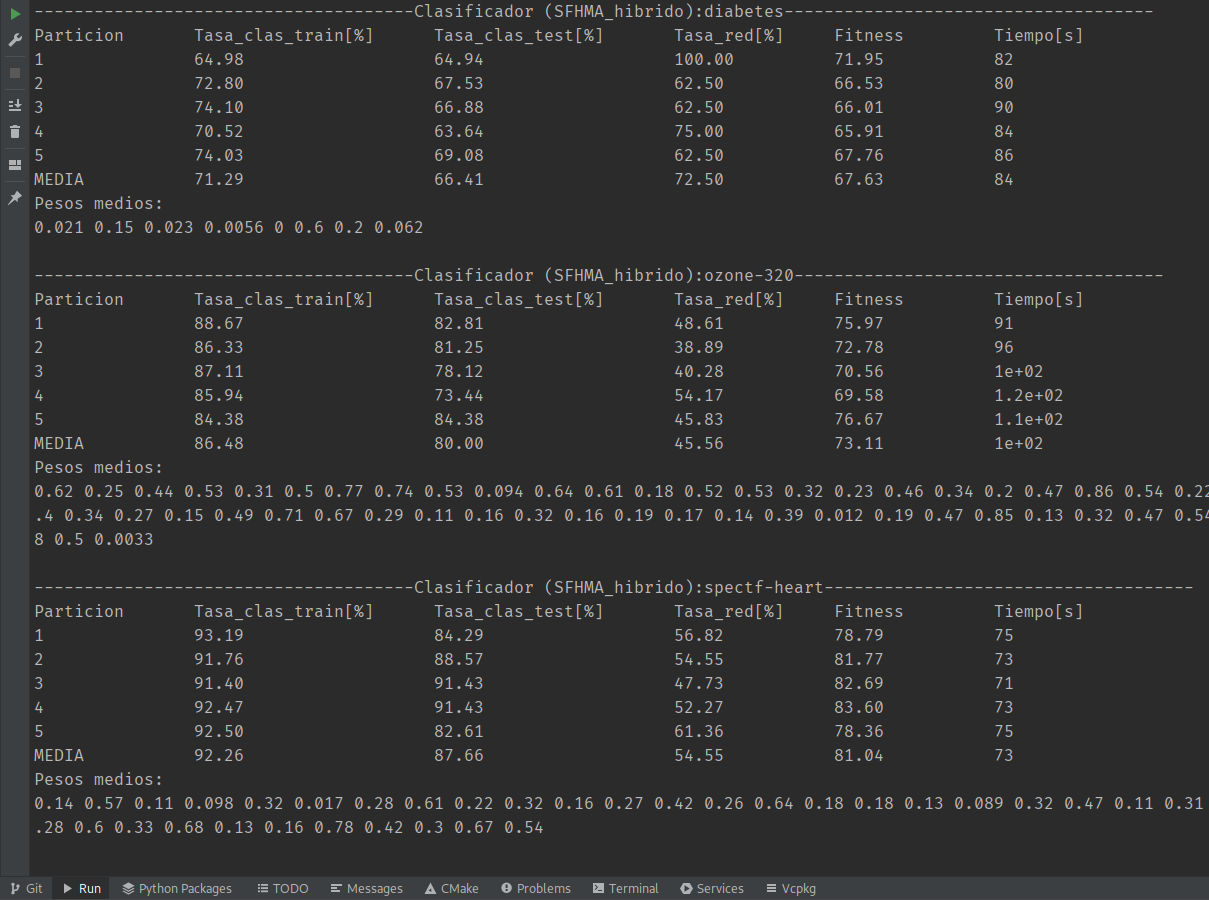
\includegraphics[width=\textwidth]{greedy.png}
	\caption{Ejecución de SFMHA}
	\label{fig:greedy}
\end{figure}
Nota: Se añade la tasa\_clas de entrenamiento para comparar en la web. Se puede desactivar quitando el parámetro \code{true} en la linea 142 en main.cpp. Para la ejecución de las tablas siguientes se ha desactivado para mejorar los tiempos. \\

\bibliography{citas} %archivo citas.bib que contiene las entradas 
\bibliographystyle{plain} % hay varias formas de citar

\end{document}
